
\section{Programs and ports}

A very basic problem that keeps cropping up in robotics projects is
simply how to move data around between sensors, processors,
and actuators.  







\subsection{The YARP Network}


\begin{figure}[t]
\centerline{
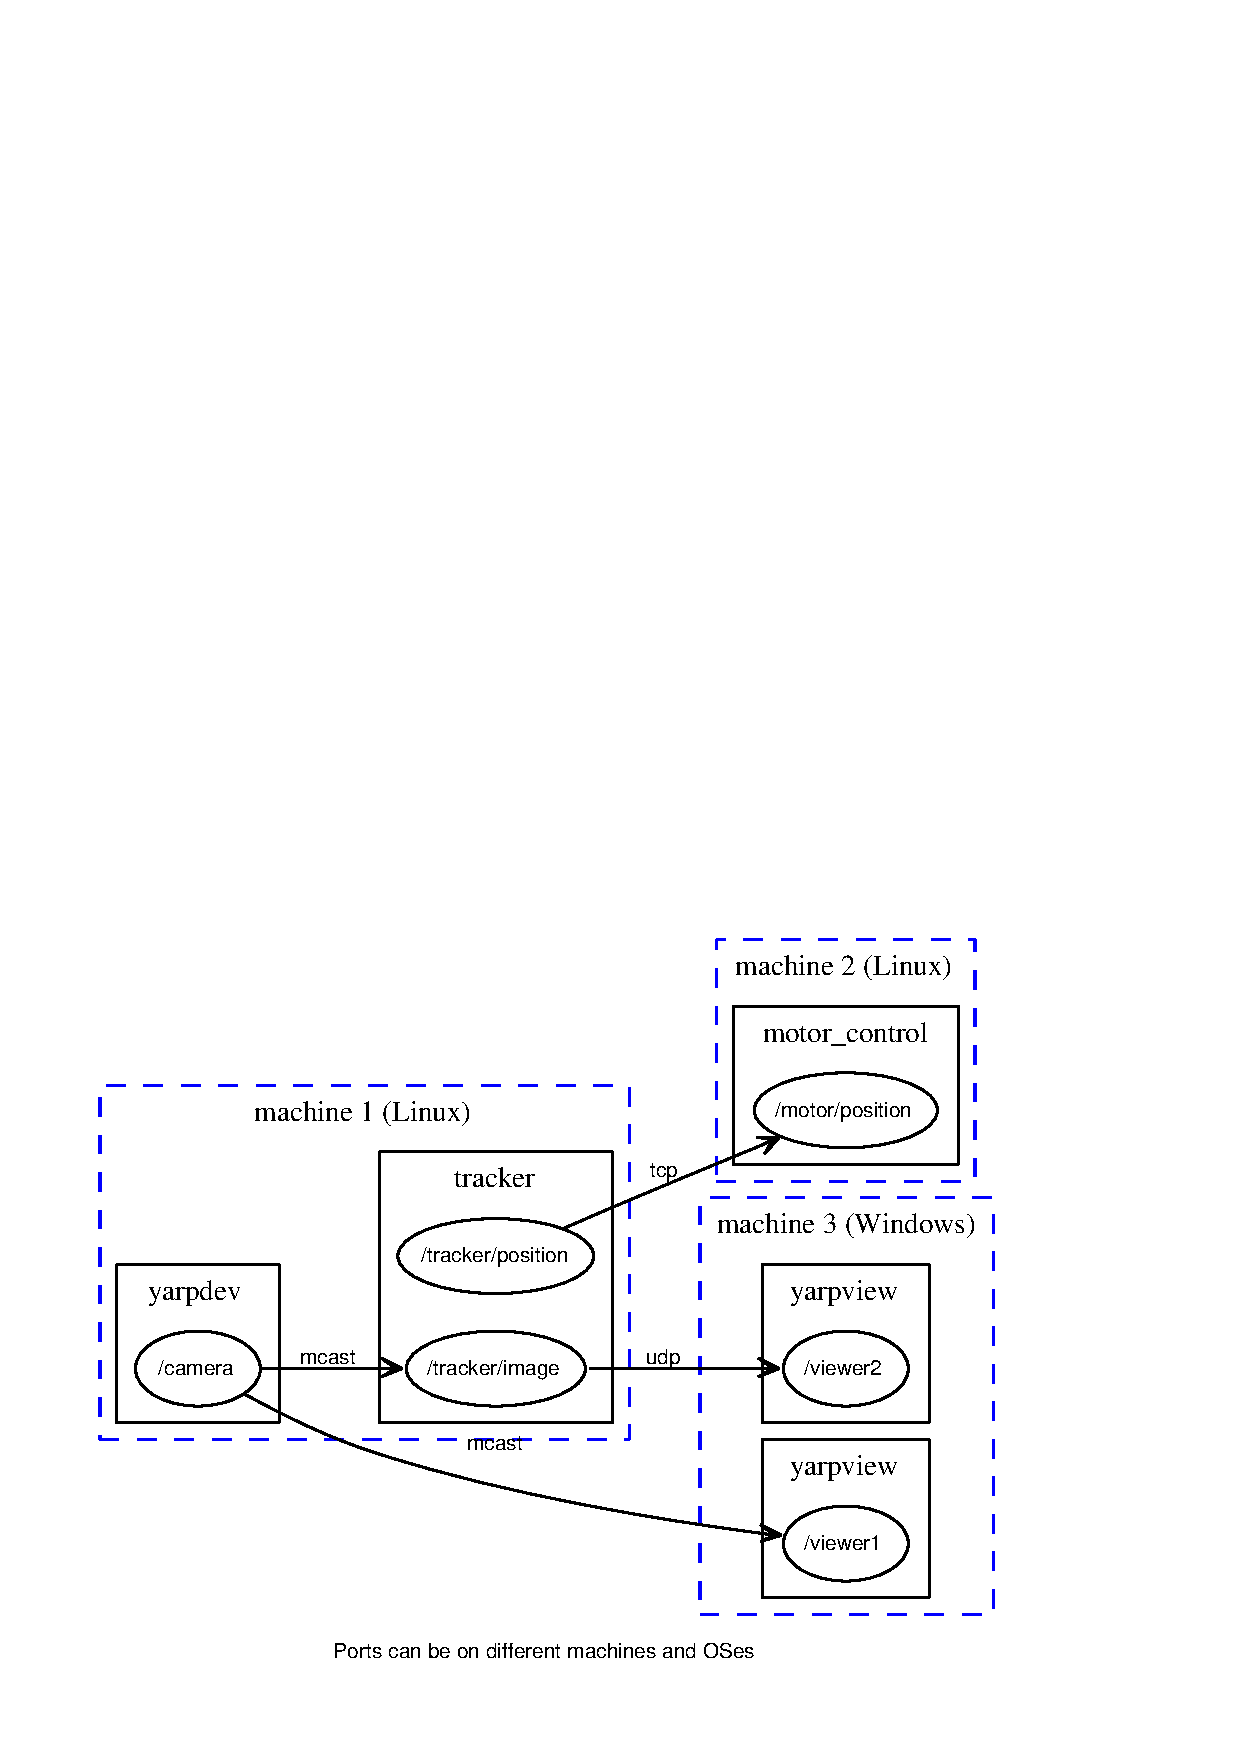
\includegraphics[width=10cm]{fig-ports}
}
\caption{
%
Port example.  Explanation.
%
}
\end{figure}


The ``YARP Network'' is built up of nodes called
``ports'' and directed edges called ``connections''.
Ports are owned by processes; many ports can belong to the same
process.  They deliver data to and from their owner.

Upon creation, by default every port communicates with a server and is
allocated a ``contact'' (an abstract address).  By default this is a
free socket port number to listen on using tcp.  The port will make
itself available for communication as directed.  Its responsibility
is only to listen for communication, and upon receiving anything
to create its side of a connection (and then immediately return 
to listening).  This is simply a generalization of a server socket.

A newly created connection is not constrained to using the
same ...





\subsection{Port abstraction}

Communication in YARP generally follows the {\it Observer} design
pattern. Special port objects deliver messages to any number of
observers (other ports), in any number of processes, distributed
across any number of machines, using any of several underlying
communication protocols. Figure XXX is a very simple network of ports
for a visual tracking application.

Images are transmitted from a camera (``/camera'') port to a viewer
(``/viewer1'') port and the input of a visual tracker
(``/tracker/image''). The tracker annotates the image, for example by
placing a marker on a tracked point, and transmits that to another
viewer (``/viewer2''). The tracker also sends just the tracked position
from a position output port (``/tracker/position'') to a input
controlling head position (``/motor/position''). Every port belongs to a
process. They do not need to belong to the same process. Every
connection can take place using a different protocol and/or physical
network. The use of several different protocol allows us to exploit
their best characteristics.
TCP is reliable, it can be used to guarantee the reception of a message.
UDP can be faster than TCP, but without guarantees.
Multicast is efficient for distributing the same information to large
numbers of targets.
Shared memory can be employed for local connections.

If messages follow YARP guidelines, then they can be
automatically converted to and from a ``text mode'' connection, for easy
human monitoring and intervention in the system.

Connections between ports in YARP can carry replies if desired,
so conventional ``RPC'' (remote procedure call) style synchronous
operation is possible.  This is a trade-off though, because this
model of communication can mske a network brittle by introducing
strong coupling of timing between processes.

This is called the YARP Network

Connections can use different protocols

Ports belong to processes

Processes can be on different machines/OS

\subsection*{Why?}

We've separated out most of the plumbing

We get to change it dynamically (handy)

More importantly, we have better modularity

Programs can be moved around as load and OS/device/library
 dependencies dictate

Fundamental protocol for communication can be changed without 
affecting programs

Better chance that your code can be used by others (even just within 
your group)



\subsection{Binary and text mode}

There is a constant tension between using binary formats and
human-readable formats.  Binary formats can be much more efficient,
but text mode formats can be much easier to work with and learn about
experimentally without extensive study.

The YARP communications system is written in two parts.  There
are a set of ``carriers'' which do the work of providing
connections between ports, so that data can be faithfully 
transmitted from a source to a destination byte-for-byte.
There is no marshalling process at this stage.

The second part of the communication system is a standard data format.
This standard is not enforced, so that the carriers could be reused by
someone with different opinions about data representation, but helper
functions and classes make it easy to meet.  This format is called the
``bottle'' format for historical reasons.  There is a general-purpose
helper class in YARP called ``Bottle'' that reads and writes data in
this format, but the format is also used by special purpose classes
such as Vector and Image.  Extensive examples are available on how
to generate data in this form.

\subsection{The bottle representation}

The bottle representation is based on a nested structure of certain
primitive types.  

Here are some informal examples of bottles, expressed in text form:

\begin{tabular}{p{5cm}p{6cm}}
10 20 30 & a list of three integers \\
10.0 20.5 31.4159 & a list of three floating point numbers \\
action "go left" (10 20 30) & a list of two strings (``action'' and ``go left''), and a nested list of integers
\end{tabular}

The structure is basically that of an s-expression
\cite{rivest1997sexp}, except that the outermost parentheses are
omitted.  This makes the important and common case of messages without
any nesting easier to write for those unfamiliar with s-expressions.
The drawback is that this means that a bottle must always be a list,
rather than any of the other primitive types, and (depending on the
input mechanism) it may also need to be non-empty.

The primitives types available are lists, integers, floating point
numbers, strings, blobs (uninterpreted sequence of bytes), and
``vocabs''.  The vocab type is the one unfamiliar type in this list.
It is motivated by the dual requirements of efficiency of machine
interpretation binary representations, and ease of human reading and
writing of text representations.  For data with a tag in it upon which
a dispatch will occur, it is simplest if that tag is a simple integer
in binary mode rather than a piece of variable-length text.
Vocabs are represented as simple integers in binary, and short
(up to four ASCII character) strings in text, with a one-to-one
mapping between the characters and bytes in the integer.  


\begin{tabular}{p{5cm}p{6cm}}
[set] [pos] 1 30.3 & a list of two vocabs, an integer, and a floating
point number -- perhaps to set the position of a specific axis.
\end{tabular}

The important point is that under normal operation, ports can be
sending fixed size messages to each other, but then when a human
eavesdrops on that data or tries to insert a message, they can still
understand and generate the identifiers being used.


The basic constraints on the design of this format were as follows:

\begin{itemize}

\item Messages in ths format should have a convenient binary and text
representation.

\item The process of translating between binary and text
representations should be mechanical, and ``round-trips'' should not
change the value significantly (except potentially with some round-off
in floating point numbers).

\item The text representation should be as easy as possible
to express from the command-line of common shells.

\end{itemize}

The reason for the last item is to make YARP messaging compatible
with typical UNIX pipe operation.  Such operation does not 
really survive well when different character encodings may be
in use, but still has uses.



character encoding issues, not yarp's concern (but clash with shell 
operation).


The structure
can be expressed in several representations.  For messaging there are:

\begin{itemize}

\item Binary form -- used for efficient messaging that is
easily machine readable/writable.

\item Text form -- used for messaging that is easily human
readable/writable (but less efficient for large messages).

\end{itemize}

It is also convenient to add two extra representations:

\begin{itemize}

\item Command-line form -- arguments to a program.

\item Configuration form -- groups and lines in a configuration file.

\end{itemize}

This is useful when dealing with configuration of devices; since
information could come from file, command line options, or across the
network, it is convenient to have all the various represenations
mapping to a homogeneous structure.



\subsection{Examples}

Capital letters are constants
(L=List, D=Double, I=Integer, S=String, B=Blob, V=Vocab).



A vector of 4 doubles.  S-expression: (1.0 -20.0 76.2 41.9).

\newcommand{\mm}{p{0.25cm}}
\newcommand{\m}{p{1cm}}
\newcommand{\md}{p{2cm}}

\begin{tabular}{|\m|\m|\md|\md|\md|\md|}
\hline
L+D & 4 & 1.0 & -20.0 & 76.2 & 41.9 \\
\hline
\end{tabular}


\subsection{Fiddling with the format}

For robotics applications that are confined to a 
local area network with all source code available,
changes to the data format are possible.

The default binary representation for integers on
the wire for YARP is little-endian.  Conversions
happen for non big-endian systems (e.g. MAC PPC).
For a network that is all big-endian,  the 
binary representation can be flipped. 

This could also be desired for XDR compatibility.
The string and blob representations also would
need to be updated to do padding which YARP does
not do.  These changes would be very narrowly
localized.

Such a modified system would lose binary-mode compatibility with any
modules using the standard YARP binary format, but connections could
still be made in text mode.

In principle, evolution of the communication protocol in YARP can be
relatively painless.  Since new ``carriers'' can be added,
modifications could be placed within a new carrier, while support for
older carriers is continued for a generation or two.  Ideally,
something like today's text mode format should be honored for a long
time, as a connection protocol of last resort.
(NOTE: this is about more than just the bottle format; reorder).


\subsection{Connection protocol}

This is the protocol used for a single connection from an output port
to an input port. It has two main phases, the handshake phase,
and the message phase.

We begin once the sender has successfully opened a bidirectional
streaming connection (think: tcp socket) to the receiver.


\subsubsection{Handshake phase}

This phase follows immediately after the connection is established.

\begin{itemize}

\item {\bf Transmission of protocol specifier}:
Sender transmits 8 bytes that identify the ``carrier'' that will be
used for the connection.  The carrier can require switching to 
some other form of stream, or using a particular strategy for
encoding data.  The transmission of the initial 8 bytes is the
only part of this protocol that is defined in terms of bytes sent.

\item {\bf Transmission of sender name}: Sender transmits the name of
the port it is associated with.  How this name is encoded and sent is
the concern of the specific carrier.

\item {\bf Transmission of extra header material}: Sender and
receiver may engage in further communication as needed for the
specific carrier.  

\end{itemize}

At the end of this phase, the sender and receiver are both ``aware''
of which carrier is in use (this may have involved discarding the
original stream and switching to a new one -- e.g. mcast, udp, shared
memory) and both are aware of the identifier of the port at the
other end of the connection.  This can be important for collaboration
during connection shutdown.


\subsubsection{Message phase}

After the handshake, the connection is (as far as YARP is concerned)
quiescent until either the sender decides to send a message across it.
It is technically possible for the receiver to initiate activity --
we'll return to this issue.

\begin{itemize}

\item {\bf Transmission of index}: Carrier-dependent. Some carriers
will require statistics about the message (such as its length) to be
given at the beginning.  YARP binary carriers have a fairly elaborate
index, due historically to a limitation of the QNX message-passing
API.  Text-mode carriers have no index at all, since it is
unreasonable to expect a human to be able to generate one.

\item {\bf Transmission of payload}: The actual message is
transmitted in a carrier-dependent way.

\item {\bf Acknowledgement of payload}: The receiver may 
acknowledge transmission in some way.  Carrier-dependent.

\end{itemize}

The message phase repeats as often as the user wants.


\subsection{What isn't carrier-dependent?}

The description so far sounds very loose -- just about every aspect
of a connection is carrier-dependent.  What does YARP actually
expect of connections, in order to build on them?

\begin{itemize}

\item After the handshaking phase, both sides of a connection know the
names of the other side.  This is important for housekeeping.

\item After the handshaking phase, a connection endpoint must have
certain knowledge about the connection that it can report to YARP.  It
will be connection-based or connectionless.  It will be text mode or
binary.  It will deliver acknowledgements or not.  It will be able to
deliver replies or not.  It will be active or ``fake'' (in multicast,
many logical connections can be serviced with a single active
connection -- these details are taken care of at the carrier level).

\end{itemize}

Before sending each message, YARP also expects the endpoint to know
whether the connection can be ``escaped'' -- that is, it can accept
port-to-port administrative communication that is not passed on as
normal user data.  The only time escaping is not desired on a carrier
is in text-mode, when the bytes transmitted should follow the user
data as slavishly as possible.  In all other cases, some
administrative data is currently packaged by YARP with user data and
then extracted at the other end.  In future carriers will be given
more control over how this material (called the ``port protocol'') is
embedded.

Everything else is convention.

\begin{tabular}{c|c|c}
\hline
8-byte magic number&protocol&variant \\\hline
`Y' `A' 0x61 0x1E 0 0 `R' `P'&udp&\\\hline
`Y' `A' 0x\-E1 0x1E 0 0 `R' `P'&udp&\\\hline
`Y' `A' 0x62 0x1E 0 0 `R' `P'&mcast&\\\hline
`Y' `A' 0x\-E2 0x1E 0 0 `R' `P'&mcast&\\\hline
`Y' `A' 0x63 0x1E 0 0 `R' `P'&shmem&\\\hline
`Y' `A' 0x\-E3 0x1E 0 0 `R' `P'&shmem&\\\hline
`Y' `A' 0x64 0x1E 0 0 `R' `P'&tcp&without acks \\\hline
`Y' `A' 0x\-E4 0x1E 0 0 `R' `P'&tcp&with acks \\\hline
`C' `O' `N' `N' `E' `C' `T' ` ' &text&without acks \\\hline
`C' `O' `N' `N' `A' `C' `K' ` ' &text&with acks \\\hline
`L' `O' `C' `A' `L' `I' `T' `Y'&local&\\\hline
\end{tabular}



\subsection{YARP without YARP}

Suppose some YARP programs are running and we want to send or
receive data from them.

For example, suppose there is a YARP system running, with a 
port called ``/motors'' which will accept commands to move a
motor.  For concreteness, let's imagine we have started the
following standard YARP programs (on the same or different 
machines):

\begin{verbatim}
yarp server
yarpdev --device test_motor --axes 2 --single_port --name /motors
\end{verbatim}

The ``yarpdev'' program here creates a port called ``/motors'' that can
accept command to a fake set of motors (2 axes or degrees of freedom),
and report on their state.

Normally we would interact with the motor through a code
interface that deals with communication.  But if for 
some reason we can't use the YARP codebase, what can
we do?

YARP ports listen to incoming tcp connections, always ready to make
new connections for input or output.  Suppose we can discover that
``/motors'' is listening on port 10022 of our current machine (we could
discover that using netstat on Linux, or by querying the YARP server
as we'll see shortly).

We can then connect manually to the port as follows:

\begin{tabular}{|l|l|}
\hline
(type in shell) & telnet 127.0.0.1 10022 \\
\hline
(type in telnet) & CONNECT foo \\
\hline
telnet responds with: & Welcome foo \\
\hline
(type in telnet) & help \\
\hline
telnet responds with: & (an explanation of available commands) \\
\hline
(type in telnet) & * \\
\hline
telnet responds with: & This is /demo at tcp://127.0.0.1:10032 ... \\
\hline
\end{tabular}

Everything so far would be basically the same for any YARP port.
For people who have used MUDs, IRC, or serial interfaces to hardware,
it should all seem vaguely familiar.

So far all our communications have been ``administrative'' --
we have communicated with the port but not really with the 
program that owns it.  To do that, we send payload data.  For the
text-mode carrier we've chosen (determined by the 8 initial
bytes we sent, ``CONNECT '' in this case), this is done by typing
``d'', hitting return, then writing a text-mode representation of
the data we want to send.  Let's try it:

\begin{tabular}{|l|l|}
\hline
(type in telnet) & d \\
\hline
(type in telnet) & help \\
\hline
telnet responds with: & (a list of possible yarpdev messages)\\
\hline
(type in telnet) & d \\
\hline
(type in telnet) & [get] [axes] \\
\hline
telnet responds with: & [is] [axes] 2 [ok] \\
\hline
(type in telnet) & d \\
\hline
(type in telnet) & [set] [pos] 0 100.0 \\
\hline
telnet responds with: & [ok] \\
\hline

\end{tabular}

We have determined that there are indeed two axes available as we requested
when starting yarpdev, and have set the position target for the
first axis to 100.0 units.  We could go on to query positions, use
other interfaces, etc.  We can disconnect by closing our connection
(or, more politely, sending the message ``q'').

By default, the motor port will stream encoder readings from the motors
to any reader that connects.  To subscribe to this stream, we simply
connect as above and then type ``r'' to reverse the connection.
Reversing means to invert which side should take the initiative
in sending data.


\begin{tabular}{|l|l|}
\hline
(type in shell) & telnet 127.0.0.1 10022 \\
\hline
(type in telnet) & CONNECT foo \\
\hline
telnet responds with: & Welcome foo \\
\hline
(type in telnet) & r \\
\hline
telnet responds with: & do \\
\hline
 & 100.0 0.0 \\
\hline
 & do \\
\hline
 & 100.0 0.0 \\
\hline
 & ... \\
\hline
\end{tabular}

The ``do'' is just like ``d'', to inform the recipient that user data
follows.  The ``o'' part means that replies are not expected by the
sender, and should not be sent.  This seems like a small detail,
but in fact when replies are not expected the performance of 
streaming to multiple targets can be greatly improved in general,
so it is worth mentioning.

Suppose we wanted to send messages more efficiently?  We start out the
same way, connecting via TCP, and then give the ``magic number'' of
the carrier we want to use (tcp binary, udp, mcast, shmem, etc).
Understanding these carriers is a bit harder than basic text-mode operation,
but logically it is all the same thing.

One part we skipped at the start was how to discover how to 
access ports in ths first place.  If we know the port we want
is called ``/motors'', how do we discover where it is?

To do that, we need to talk to the ``yarp server'', which is analogous
to a standard DNS name server.  If we're using YARP, our program would
be able to discover where the server is by itself (by checking
standard configuration files if available or sending broadcast
messages if necessary).  Or, if we don't want to use yarp at all, we
can simply make a note of what machine and port number it is running
on.  Suppose it is on 127.0.0.1 listening to port number 10000.
We can communicate with the name server exactly as with any regular
port.

\begin{tabular}{|l|p{8cm}|}
\hline
(type in shell) & telnet 127.0.0.1 10000 \\
\hline
(type in telnet) & CONNECT foo \\
\hline
telnet responds with: & Welcome foo \\
\hline
(type in telnet) & d \\
\hline
(type in telnet) & help \\
\hline
telnet responds with: & (an explanation of available name server commands) \\
\hline
(type in telnet) & d \\
\hline
(type in telnet) & query /motors \\
\hline
telnet responds with: & registration name /motors ip 127.0.0.1 port 10022 type tcp \\
\hline
\end{tabular}

So we now know how to reach /motors (tcp connection to 127.0.0.1 port 10022).
%
So, with a running YARP system, we have seen how to discover
and communicate with running programs, sending commands and reading
data, without using any YARP libraries or executables.  All the steps
we've gone through are trivial in any language with a basic socket
library (we're not using any special features of telnet, it is just
for demonstration purposes).  It is important to remember, though,
that while we've been communicating with the ``/motors'' port using
text across tcp, at the same time the same port could be communicating
with other programs via binary messages over udp or multicast etc.


%What if we wanted to make a port ourselves?  To make a full-featured
%port supporting all the carriers that YARP does would be quite a lot
%of work.  To make a basic port that just supports text-mode tcp
%communication is easier.  A demo is a little cumbersome for this paper...


\subsection{Problems}

Not localization friendly, English bias at a quite low level.
Probably localization would not be practical at the network
protocol level.  Also approach to character encoding is
primitive and ad-hoc; no guarantee that encoded data
will survive in text-mode.


\subsection{Other bits}

YARP is a free and open source project.  Since its source code is
released under a free and open license, useful parts of it can be used
by other systems, and its operation can be studied.

YARP has a large quantity of documentation (although we always need
more).  The communication protocol it uses is documented, and can be
interfaced with without using the YARP code-base.

Beyond just documenting the communication protocol, particular attention
has been devoted to make sure that that reading and writing data to a
YARP port can be done with very little effort.  YARP ports will 
accept and make connections of any of several different forms;
for a program build without the YARP code-base, it suffices
to implement just one of those connection types in order to
get basic connectivity.  If bandwidth requirements are not
excessive, the very simplest connection type can be implemented:
a very basic text-mode protocol.

